\section{Data space estimators} \label{sec:ClosureEstimators}

\subsection{Deriving the data space estimators}
\label{sec:ClosureEstimatorsDerivation}

We start by defining the model error as the expectation across models of the
$\chi^2$ between the model predictions and some data central values
$\testset{\obspriorcent}$, normalised by the number of data points
\begin{equation}
    \label{eq:chi2kerep}
    \eout = \frac{1}{\ndata} \emodel{
        \left( \testset{\fwdobsop}\left(\modelvecrep\right) - \testset{\obspriorcent} \right)^T
        \testset{\obspriorcov}^{-1}
        \left( \testset{\fwdobsop}\left(\modelvecrep\right) - \testset{\obspriorcent} \right)
    }\, ,
\end{equation}
where we defined the expectation value over the ensemble of model replicas as
\begin{equation}
    \emodel{\cdot} \equiv \frac{1}{\nreps} \sum_{k=1}^{\nreps} \cdot \, ,
\end{equation}
and we purposely denoted the data which the model error is evaluated on as
$\testset{\obspriorcent}$, as opposed to the data which is used to determine the model
parameters $\obspriorcent$. We could of course set
$\testset{\obspriorcent} = \obspriorcent$ and
evaluate the model performance on the fitted data however, as is common in
machine learning literature, we intend to use a separate set of test data.
Ideally we would choose $\testset{\obspriorcent}$ such that the joint prior
distribution of training and test set can be written as
$\pi_{D}^0(\testset{\obspriorcent}, \obspriorcent) =
\pi_{D}^0(\testset{\obspriorcent})\pi_{D}^0(\obspriorcent)$, in other words the
training and test set are statistically independent. If the prior distribution
in data-space is Gaussian, then the total covariance of the prior would be
block diagonal in the training and test covariance:
\begin{equation}
    \modelpriorcov^{\rm Total} =
    \begin{bmatrix}
        \modelpriorcov  & 0  \\ 
        0  & \testset{\modelpriorcov}  \\ 
    \end{bmatrix}
\end{equation}
In the
context of a closure test, $\eout$ is a stochastic quantity which depends both
on the training data, through the ensemble of MAP estimators, and the test data.

It is useful perform a decomposition of this expression, a similar exercise is
performed for the likelihood function associate with least-squares regression in
\cite{mlforphysics}. Least-squares regression is a special case of minimum
likelihood estimation, where the uncertainty on each data point is equal in
magnitude and uncorrelated. Here we review the decomposition in the more general
framework of data whose uncertainty is multigaussian. Starting with
Eq.~\ref{eq:chi2kerep} (evaluated on the ideal test data), we can complete the
square
\begin{equation}
    \begin{split}
    \label{eq:EoutDecomposition}
        &\eout = \frac{1}{\ndata} \emodel{
            \left( \testset{\fwdobsop}\left(\modelvecrep\right) - \testset{\law} \right)^T
            \testset{\obspriorcov}^{-1}
            \left( \testset{\fwdobsop}\left(\modelvecrep\right) - \testset{\law} \right)
        } + \\
        &+ \emodel{
            \left( \testset{\law} - \testset{\obspriorcent} \right)^T
            \testset{\obspriorcov}^{-1}
            \left( \testset{\law} - \testset{\obspriorcent} \right)
        }+ \\
        &+ 2 \emodel{
            \left( \testset{\fwdobsop}\left(\modelvecrep\right) - \testset{\law} \right)^T
            \testset{\obspriorcov}^{-1}
            \left(\testset{\law} - \testset{\obspriorcent} \right)
        }\, .
    \end{split}
\end{equation}
The second term is the shift associated with evaluating the model error on
noisey test data and the final term is a cross term which we will deal with
later. We can decompose the first term further,
% TODO: add the same thing but for fully in sample data to an appendix.
\begin{equation}
    \begin{split}
        &\emodel{
            \left( \testset{\fwdobsop}\left(\modelvecrep\right) - \testset{\law} \right)^T
            \testset{\obspriorcov}^{-1}
            \left( \testset{\fwdobsop}\left(\modelvecrep\right) - \testset{\law} \right)
        } = \\
        &= \emodel{
            \left( \testset{\fwdobsop}\left(\modelvecrep\right) - 
            \emodel{\testset{\fwdobsop}\left(\modelvecrep\right)} \right)^T
            \testset{\obspriorcov}^{-1}
            \left( \testset{\fwdobsop}\left(\modelvecrep\right) - 
            \emodel{\testset{\fwdobsop}\left(\modelvecrep\right)} \right)
        } + \\
        &+ \left( \emodel{\testset{\fwdobsop}\left(\modelvecrep\right)} - \testset{\law} \right)^T
        \testset{\obspriorcov}^{-1}
        \left( \emodel{\testset{\fwdobsop}\left(\modelvecrep\right)} - \testset{\law} \right)\, ,
    \end{split}
\end{equation}
where we have used the fact that the second term is constant across replicas and
the cross term that arises in this decomposition is zero when the expectation
value across replicas is taken. The first term in this expression we call the
{\em variance} and the second term is the {\em bias}.

As previously mentioned $\eout$ should be considered a stochastic estimator, in
theory we could take the expectation value across training data $\obspriorcent$ and
test data $\testset{\obspriorcent}$, the latter of which cancels the cross term in
Eq.~\ref{eq:EoutDecomposition}. The final result of that would be
\begin{equation}\label{eq:ExpectedBiasVariance}
    \mathbf{E}_{\obspriorcent, \testset{\obspriorcent}}[\eout] =
    \mathbf{E}_{\obspriorcent}[{\rm bias}] + 
    \mathbf{E}_{\obspriorcent}[{\rm variance}] +
    \mathbf{E}_{\testset{\obspriorcent}}[{\rm noise}]\, .
\end{equation}
We are not interested in the observational noise term, since it is
independent of the model and in the limit of infinite test data
$\mathbf{E}_{\testset{\obspriorcent}}[{\rm noise}] \to 1$.
The two estimators of interest are independent of
the test data, and therefore we only need to take the expectation value over
the training data.

\paragraph{Multiple closure fits}
In practical terms, taking the expectation value across the training data can
be achieved by running multiple closure fits, each with a different
observational noise vector $\obsnoise$, and taking the average i.e.
\begin{equation}
    \mathbf{E}_{\modelpriorcent}[ \cdot ] = \frac{1}{\nfits} \sum_{j=1}^{\nfits} \cdot.
\end{equation}
Clearly this is resource intensive, and requires us to perform many fits. In
NNPDF3.0 \cite{nnpdf30}, single replica proxy fits were used to perform a study
of the uncertainties. Here we have expanded the data-space estimators used in
the closure fits and also will be using multiple full replica fits to
calculate various expectation values - made possible by our next generation
fitting code.

\subsection{Geometric Interpretation}

It is possible to interpret the relevant data space estimators geometrically, by
considering a coordinate system where each basis vector corresponds to an
eigenvector of the experimental covariance matrix normalised by the square root
of the corresponding eigenvalue. The origin of the coordinate system is the true
value of the observable. The model predictions are then a set of points, where
the mean squared radius of those points is what we call the variance. The bias
is the l2-norm of the vector between the origin and the mean of the model
predictions. An example of this is given in Fig.~\ref{fig:diagram2destimators},
where for simplicity we have considered a system with just two data points, \ie\
a two-dimensional data space, with a diagonal covariance.
%
\begin{figure}
    \centering
    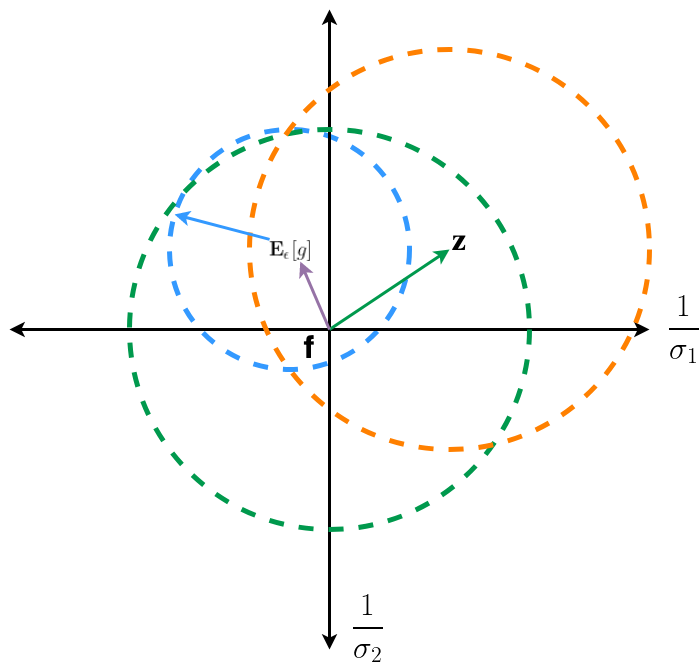
\includegraphics[width=0.8\textwidth]{diagonal_basis_2d_estimators_diagram.png}
    \caption{Example of geometric interpretation of closure test estimators.
    The origin
    is the true observable values for each data point. The level one data (or
    experimental central values) are
    shifted away from this by $\obsnoise$. In this example the covariance matrix
    is diagonal, so the eigenvectors correspond to the two data points, the
    square root of the eigenvalues are simply the standard deviation of those
    points. This is without loss of generality because any multivariate distribution
    can be rotated into a basis which diagonalises the covariance matrix.
    The 1-sigma observational noise confidence interval
    is a unit circle centered on the origin. Some closure
    estimators can be understood as l2-norms of the vectors connecting points,
    i.e the bias is the l2-norm of the vector from the origin to the central
    value of the predictions.}
    \label{fig:diagram2destimators}
\end{figure}
%

\subsection{Faithful uncertainties in data space}

The two closure estimators of interest, bias and variance, can be used to
understand faithful uncertainties in a practical sense. If we return to
Eq.~\ref{eq:ExpectedBiasVariance} we can examine both estimators in a bit more
detail.

\paragraph{Variance}

The {\em variance} in the above decomposition refers to the variance of the
model predictions in units of the covariance
\begin{equation}
    \label{eq:VarDef}
    \begin{split}
        % NOTE: not using \emodel here in order to split line.
        \var &= \frac{1}{\ndata}\mathbf{E}_{\{ \modelvec_* \}} \Big[ \\
            &\left( \testset{\fwdobsop}\left(\modelvecrep\right) - 
            \emodel{\testset{\fwdobsop}\left(\modelvecrep\right)} \right)^T
            \testset{\obspriorcov}^{-1}
            \left( \testset{\fwdobsop}\left(\modelvecrep\right) - 
            \emodel{\testset{\fwdobsop}\left(\modelvecrep\right)} \right)
        \Big] \, ,
    \end{split}
\end{equation}
which can be interpreted as the model uncertainty in the space of the test data.
It is instructive to rephrase Eq.~\ref{eq:VarDef} as
\begin{equation}
    \label{eq:VarDefalternative}
    \var = \frac{1}{\ndata} {\rm Tr} \left[ \covrep \testset{\obspriorcov}^{-1} \right],
\end{equation}
where 
\begin{equation}
    \label{eq:CovRep}
    \covrep = 
    \emodel{
            \left( \testset{\fwdobsop}\left(\modelvecrep\right) - 
            \emodel{\testset{\fwdobsop}\left(\modelvecrep\right)} \right)
            \left( \testset{\fwdobsop}\left(\modelvecrep\right) - 
            \emodel{\testset{\fwdobsop}\left(\modelvecrep\right)} \right)^T
        }
\end{equation}
is the covariance matrix of the predictions from the model replicas. Note that
we can rotate to a basis where $\testset{\obspriorcov}$ is diagonal,
\begin{equation}
    \label{eq:InvCovPrimeDiag}
    \left(\testset{\obspriorcov}^{-1} \right)_{ij} = \frac{1}{\left(\testset{\sigma}_i\right)^2} 
    \delta_{ij}\, ,
\end{equation}
then we can rewrite Eq.~\ref{eq:VarDefalternative} as 
\begin{equation}
    \label{eq:VarianceInterpretation}
    \var = \frac{1}{\ndata}\, \sum_i \frac{\covrep_{ii}}{\left(\testset{\sigma}_i\right)^2}\, .
\end{equation}
The numerator in the right-hand side of the equation above is the variance of
the theoretical prediction obtained from the fitted replicas, while the
denominator is the experimental variance, the average is now taken over
eigenvectors of the experimental covariance matrix.

% The following needs to be reworded or removed, the use of prior and posterior
% here is confusing because the prior here is nothing to do with the prior
% of the training data but the posterior is only the posterior of the training
% data and instead is the prior of the model when considering the test data..

% If the replicas are sampled from the
% posterior distribution of model, the right-hand side of the
% equation is the average reduction in the variance of the observables between the
% prior distribution, dictated by the experimental covariance, and the posterior
% distribution. The average is computed over the space of test data, \ie\ data
% points that are not seen by the fit. 

\paragraph{Bias}

Similarly, the {\em bias}\ is defined as the difference between the expectation
value of the model predictions and the true observable values in units of the
covariance, \ie 
\begin{equation}
    \label{eq:BiasDef}
    \bias = \frac{1}{\ndata}
    \left( \emodel{\testset{\fwdobsop}\left(\modelvecrep\right)} - \testset{\law} \right)^T
    \testset{\obspriorcov}^{-1}
    \left( \emodel{\testset{\fwdobsop}\left(\modelvecrep\right)} - \testset{\law} \right)\, .
\end{equation}
The smaller the bias, the closer the central value of the predictions is to the
underlying law. In Eq.~\ref{eq:ExpectedBiasVariance}, the expectation value is
taken across the prior distribution of the training data, which yields
\begin{equation}
    \mathbf{E}_{\obspriorcent}[{\rm bias}] = \frac{1}{\ndata}
    {\rm Tr} \left[ \covcent \testset{\obspriorcov}^{-1} \right]\, ,
\end{equation}
where we have introduced $\covcent$ as the covariance of the expectation value
of the model predictions,
\begin{equation}
    \label{eq:CovCentDef}
    \covcent = 
    \mathbf{E}_{\obspriorcent}\left[
        \left( \emodel{\testset{\fwdobsop}\left(\modelvecrep\right)} - \testset{\law} \right)
        \left( \emodel{\testset{\fwdobsop}\left(\modelvecrep\right)} - \testset{\law} \right)^T   
    \right]\, .
\end{equation}
The point is that the bias on the test data is a stochastic variable which
depends on the central value of the training data through $\modelvecrep$. The
matrix $\covcent$ describes the fluctuations of the central value of the model
prediction around the true observable values as we scan different realisations
of the training data. 

It is important to stress the difference between variance and bias. In the case
of the variance, we are looking at the fluctuations of the replicas around their
central value for fixed $\obspriorcent$. This is related the ensemble of model
replicas we provide as the end product of a fit and can be calculated when
we have one instance of $\obspriorcent$, provided by the experiments.
In the case of the bias we consider the flucutations of the central value over
replicas around the true theoretical prediction as the values of $\obspriorcent$
fluctuate around $\law$. This latter procedure is only possible in a
closure test, where the underlying true observable is known. The
bias as defined here yields an estimate of the fluctuations of the MAP estimator
if we could do multiple independent experiments.

\paragraph{Bias-variance ratio}

Finally, the {\em bias-variance ratio} is defined as
\begin{equation}
    \label{eq:RatioDef}
    \biasvarratio \equiv \sqrt{\frac{
        \mathbf{E}_{\obspriorcent}[ \bias ]}{
            \mathbf{E}_{\obspriorcent}[ \var ]}}\, ,
\end{equation}
where we have taken the square root, since bias and variance are both mean
squared quantities. The value of $\biasvarratio$ yields a measurement of how
much uncertainties are over or under estimated. If the uncertainties are
completely faithful, then $\biasvarratio = 1$. We note that the relationship
does not work both ways and $\biasvarratio = 1$ does not necessarily guarantee
that the uncertainty is faithful. We also note that $\biasvarratio$ is not
completely general: it is not a measure defined in model space and depends on
the choice of test data. Therefore it only gives 'local' information on the
model uncertainties. If the distribution of the expectation value of model
predictions is gaussian centered on the true observable values, with covariance
$\covcent$ and the distribution of the model replicas is also gaussian, with
covariance $\covrep$ then model uncertainties are faithful if
\begin{equation}\label{eq:IdealRatioDef}
    \covcent {\covrep}^{-1} = 1.
\end{equation}
The difficulty with calculating Eq.~\ref{eq:IdealRatioDef} comes from the fact
that $\covrep$ is likely to have large correlations which would lead it to be
singular or ill-conditioned. As a result, any error estimating $\covrep$ from
finite number of replicas could lead to unstable results. $\biasvarratio$
overcomes this instability by taking the ratio of the average across test data
of these matrices, in units of the experimental covariance matrix. There may
still be large relative errors for smaller eigenvalues of $\covrep$, but these
should not lead to instabilities in $\biasvarratio$ unless they correspond to
directions with very low experimental uncertainty. As an extra precaution, we
shall estimate an uncertainty on $\biasvarratio$ by performing a bootstrap
sample on fits and replicas.

\paragraph{Quantile statistics}
\label{sec:QuantileStatistics}

When the closure test was first presented in \cite{nnpdf30}, there was an estimator
introduced in the space of PDFs which also aimed to estimate faithfulness of
PDF uncertainties using the combined assumption of Gaussian PDF uncertainties
and quantile statistics, called $\xi_{1\sigma}$. Here we can define an
analagous expression in the space of data,
\begin{equation}
    \label{eq:XiDataDef}
    \xisigdat{n} = 
        \frac{1}{\ndata} \sum_{i}^{\ndata} 
        \frac{1}{\nfits} \sum_{l}^{\nfits}
            I_{[-n \testset{\sigma}_i^{(l)}, n \testset{\sigma}_i^{(l)}]}
            \left( \emodel{\testset{\fwdobsop}_i}^{(l)} - \testset{\law}_i \right),
\end{equation}
where $\testset{\sigma}_i^{(l)} = \sqrt{\covrep_{ii}}$ is the standard deviation of the
theory predictions estimated from the replicas of fit $l$ and $I_{[a, b]}(x)$
is the indicator
function, which is one when $a \leq x \leq b$ and zero otherwise. In other
words, $\xisigdat{n}$ is counting how often the difference between the prediction
from the MAP estimator and the true observable value is within the $n\sigma$
confidence interval of the replicas, assuming they're Gaussian. Since $\covrep$
is primarily driven by the replica
fluctuations, we assume that it is roughly constant across fits, or independent
upon the specific instance of observational noise. Also when taking the expectation
value across fits, we're implicitly taking the expectation value across
the prior distribution of the fitted data. This allows us to write
$\xisigdat{n}$ for a specific data point in the limit of infinite fits, each to
a different instance of the data as
\begin{equation}
    \label{eq:XiIExpecVel}
    \xisigdati{n} =
    \int_{-\infty}^{\infty} I_{[-n \testset{\sigma}_i, n \testset{\sigma}_i]}\,
    \left( \emodel{\testset{\fwdobsop}_i}^{(l)} - \testset{\law}_i \right) 
    \pi_{D}^0(\obspriorcent) \, 
    {\rm d}(\obspriorcent) \, ,
\end{equation}
where $\emodel{\fwdobsop_i}^{(l)}$ has implicit conditional dependence on
$\obspriorcent$. If
the distribution of $\emodel{\testset{\fwdobsop}_i}^{(l)} - \testset{\law}_i$
is Gaussian, centered on
zero, we can defined ${\testset{ \hat{\sigma} }}_i = \sqrt{\covcent_{ii}}$. In which case
\begin{equation}
    \label{eq:expectedxi}
    \xisigdati{n} =
    \erf \left( \frac{n \testset{\sigma}_i}{\testset{\modelstd}_i \sqrt{2}}\right),
\end{equation}
which is simply the standard result of integrating a gaussian over some finite
symmetric interval.

The analogy between $\biasvarratio$ and $\xisigdat{n}$ is clear, the ratios of
uncertainties are both attempts to quantify Eq.~\ref{eq:IdealRatioDef} whilst keeping
effects due to using finite statistics under control. Whilst with
$\biasvarratio$ we take the average over
test data before taking the ratio, $\xisigdat{n}$ instead takes the ratio
of the diagonal elements - ignoring correlations. Since the predictions
from the model will be compared with experimental central values, taking into
account experimental error, we find it more natural to calculate $\xisigdat{n}$
in the basis which diagonalises the experimental covariance of the test data as
in Eq.~\ref{eq:InvCovPrimeDiag}. If we assume that in this new basis, that
both $\frac{\covrep_{ii}}{\left(\sigma'_i\right)^2}$ and
$\frac{\covcent_{ii}}{\left(\sigma'_i\right)^2}$ are approximately constant
for all eigenvectors of the experimental covariance matrix, then we recover the
approximation
\begin{equation}\label{eq:CompareXiRatio}
    \xisigdat{n} \sim \erf \left( \frac{ n\biasvarratio}{\sqrt{2}} \right).
\end{equation}
Whilst it's clear Eq.~\ref{eq:CompareXiRatio} is reliant on a fair few
assumptions which may not hold, we will use the comparison of $\xisigdat{n}$ with
$\biasvarratio$ to consider how valid these assumptions may be.
